\chapter{Syntax parameters}

Syntax parameter are a mechanism for rebinding a macro definition with the dynamic extent of a macro expansion. With syntax parameter instead of introducing the unhygienic binding each time we instead create binding for the keyword, which we can adjust later when we want the keyword to have different meaning. As no new binding is introduced so hygiene is preserved, This is similar to the dynamic binding mechanism that we have at run time, except that the dynamic binding only occurs during macro expansion.

\section{Approach 1}

In this approach I tried to use pre-processing approach similar to C, where I transform the code before the main compiler get hold of it. “SyntaxParameter” which replace and bind the parameter with  mapped value in the particular defined macro scope. Here macro transformation happen during the parse phase by matching the pattern. To define syntax parameter in Sweet.js provide a new keyword that look something like this:  

SyntaxParameter(<parameter>,<Mapped to>,<Scope/Macro Name>,<Macro definition>)
\newpage
Example of usage is shown below 

\begin{figure}[htb]
\centering
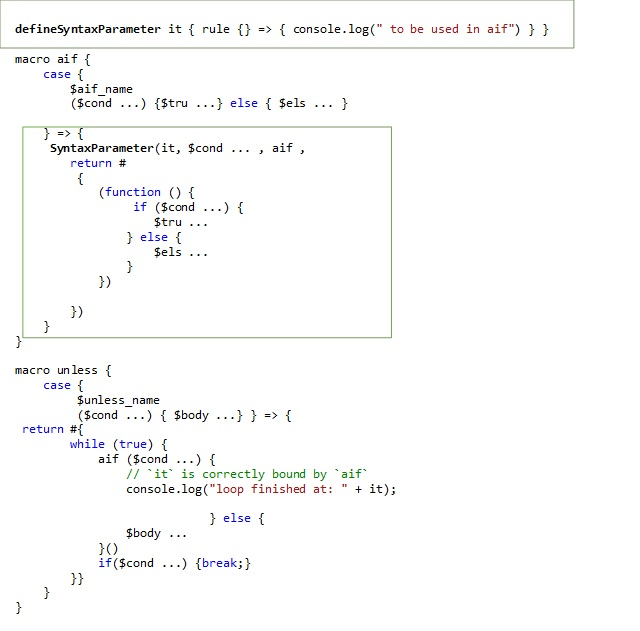
\includegraphics[width=1.0\textwidth]{images/Appraoch1.jpg}
\caption{Approach 1.} 
\label{fig:AST}

\end{figure}

\begin{figure}[htb]
\centering
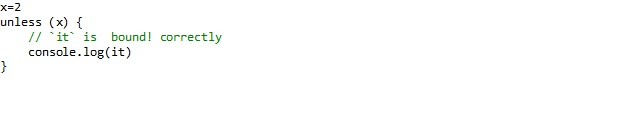
\includegraphics[width=1.0\textwidth]{images/Appraoch2.jpg}
\caption{Calling unless macro} 
\label{fig:AST}

\end{figure}

On expansion above macro looks like this

\begin{figure}[htb]
\centering
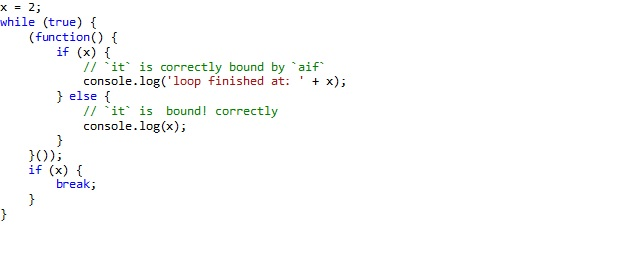
\includegraphics[width=1.0\textwidth]{images/Appraoch3.jpg}
\caption{ it identifier is correctly bounded to \$cond.. Of an anaphoric-if} 
\label{fig:AST}

\end{figure}

Since, `it' is correctly bounded to \$cond.. as desired, but this approach has certain disadvantage, since this won`t allow user to define macros with name ``SyntaxParameter'' consider like

\begin{lstlisting}[frame=single]
macro SyntaxParameter {
  ...
}
\end{lstlisting}

So to fix this we first need to implement some primitive function that help us to create and manipulate the arbitrary compile time syntax transformation. Macros are compile time syntax transformation ,At the moment in Sweet.js the only way to create a syntax transformer is by defining a macro. A macro is really just a function that takes syntax and returns syntax (thus a syntax transformer). So when the ``expander'' encounters a macro definition it converts the body of the macro into a function and loads it into the compile time environment.

\newpage
\section{Approach 2}

In this approach I, defined ``syntaxparam'' similar to define-syntax-parameter in Scheme, which load the primitive function in compile time environment,''syntaxLocalValue,'' which return the compile time value from the environment and ``replaceSyntaxParam,'' which transform the identifier with the compile time value from the environment within the specified scope of the macro. Example shown below

\begin{figure}[htb]
\centering
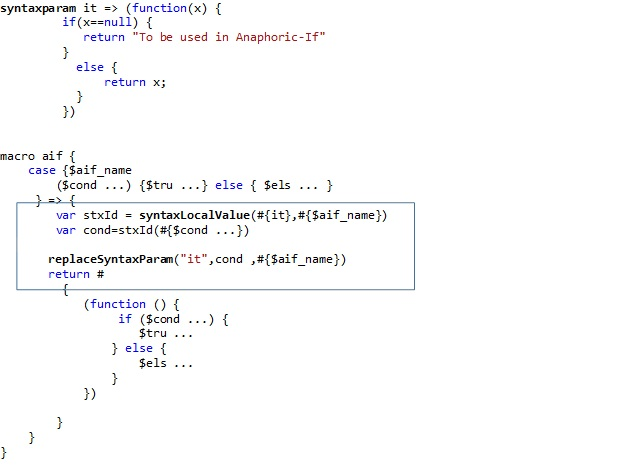
\includegraphics[width=1.0\textwidth]{images/Appraoch21.jpg}
\caption{ Approach 2.Syntax parameter implementation} 
\label{fig:AST}
\end{figure}

\begin{figure}[htb]
\centering
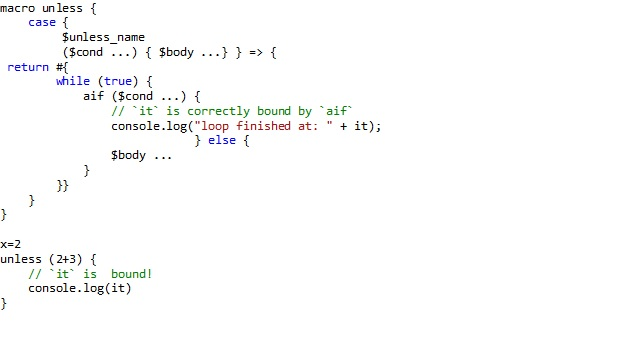
\includegraphics[width=1.0\textwidth]{images/Appraoch23.jpg}
\caption{ Approach 2.Syntax parameter implementation contd..} 
\label{fig:AST}
\end{figure}
 
\begin{figure}[htb]
\centering
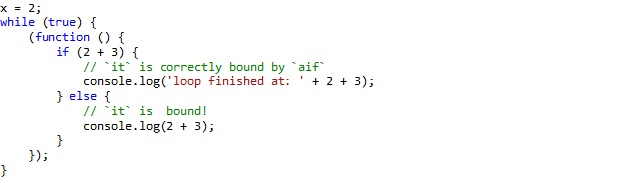
\includegraphics[width=1.0\textwidth]{images/Appraoch22.jpg}
\caption{ Approach 2. Syntax parameter expansion} 
\label{fig:AST}
\end{figure}

\newpage
\begin{figure}[htb]
\centering
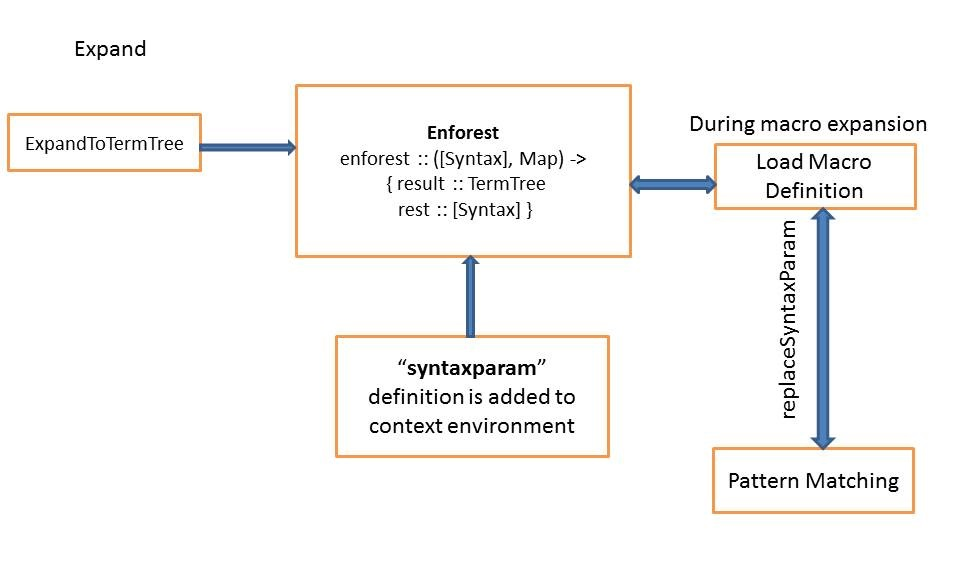
\includegraphics[width=1.0\textwidth]{images/CodeWorking.jpg}
\caption{ Approach 2. Implementation } 
\label{fig:AST}
\end{figure}

The main entry point into the expander is appropriately enough,
expand function is primarily responsible for handling hygiene. The env param is a mapping from identifier to macro definitions and ctx is a mapping of names to names. The expand function delegates to expandToTermTree, responsible for converting the syntax to TermTrees and loading any macro definitions it finds into the new env map.

Its in the ``expandToTermTree,'' it call enforest repeatedly until the entire token tree has been converted into a term tree. its in enforest function where ``syntaxparam'' definition loaded to context env map. When macro call is invoked it load the macro definition from the env in ``loadmacrodef'' function and during pattern matching ``replaceSyntaxParam'' which bind the identifier with the value.